%license:BSD-3-Clause
%copyright-holders:Michele Maione
%============================================================
%
%	Piattaforma di cloud gaming per giochi arcade
%
%============================================================

\chapter{Architettura del sistema}
In questo capitolo ...

\section{Sistema proposto}
Le caratteristiche principali del progetto, che sono state vincolanti nella scelta delle tecnologie da utilizzare, sono la portabilità e la possibilità di utilizzare il sistema senza dover installare software aggiuntivi, e per questi vincoli lato client la scelta è ricaduta sul browser web. Le tecnologie di streaming per i browser web ad oggi sono: WebSocket, HLS, DASH e WebRTC\cite{Audio_and_video_delivery}.

WebSocket è un protocollo di comunicazione che fornisce un canale full-duplex su una singola connessione TCP, con una latenza inferiore rispetto ad HLS e DASH.

HTTP Live Streaming (HLS) è il protocollo di streaming ad alta latenza più popolare su protocollo HTTP per video on demand (video preregistrato) sviluppato da Apple.

Dynamic Adaptive Streaming over HTTP (DASH) è una tecnica di streaming con bit-rate adattivo del Moving Picture Experts Group (MPEG), che consente lo streaming di alta qualità di contenuti multimediali su protocollo HTTP.

Web Real-Time Communication (WebRTC) è un progetto per la comunicazione in tempo reale basato sul protocollo RTP (Real-time Transport Protocol)\cite{High_Performance_Browser_Networking}.

\begin{figure}[H]
	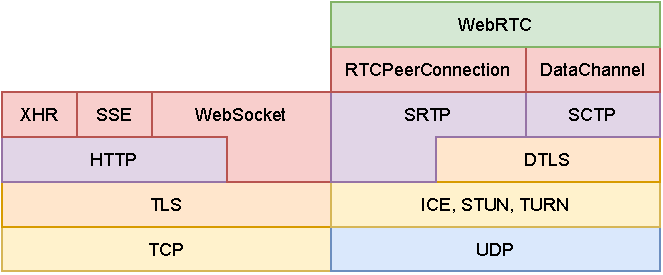
\includegraphics[width=\linewidth]{immagini/webprotocols}
	\caption{API, protocolli e servizi di rete del browser di alto livello}
	\label{fig:webprotocols}
\end{figure}

L'esigenza per la quale nasce questo progetto è far conoscere alle nuove generazioni i videogiochi che hanno fatto la storia e dare la possibilità di poter giocare ancora a macchine che ormai hanno cessato di funzionare per motivi di obsolescenza, e proprio per questo la progettazione si è basata, sì sullo streaming via rete, ma con un'ottica incentrata sull'utilizzo in stand di retro-gaming in eventi relativi all'informatica e ai videogiochi, quindi sulla rete locale dell'evento con gli utenti connessi tramite WiFi. In quest'ottica la differenza di velocità tra TCP e RTP è trascurabile, e la scelta è ricaduta su WebSocket perché è un protocollo di comunicazione standardizzato dal 2011, è pienamente supportato da tutti i browser moderni, è semplice e non richiede l'utilizzo di protocolli aggiuntivi o configurazioni complesse a differenza di WebRTC.

\begin{figure}[H]
	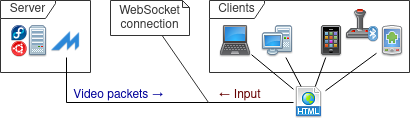
\includegraphics[width=\linewidth]{immagini/proposed_system}
	\caption{Panoramica del sistema}
	\label{fig:proposed_system}
\end{figure}

Come mostrato in Fig. \ref{fig:proposed_system} il sistema è costituito dal server di gioco, che può essere Linux, Windows o macOS, su cui è in esecuzione la versione modificata di MAME, e una pagina HTML5 che funge da front-end. Il programma è in ascolto per connessioni WebSocket con parametri (per es.: il nome del gioco, l'ID del player, l'ID della partita). Una volta stabilita la connessione, il server invia informazioni sulla dimensione e le proporzioni del video e avvia il gioco. Il rendering e il missaggio audio del gioco vengono generati tramite SDL\footnote{SDL: Simple DirectMedia Layer, una libreria multipiattaforma ed open-soure per il multimedia}, codificati e pacchettizzati in MPEG-TS\footnote{MPEG-TS: MPEG transport stream, è un contenitore digitale per la trasmissione e l'archiviazione audio-video.} tramite FFmpeg\footnote{FFmpeg è una suite open-source di librerie e programmi per la gestione di video, audio, e altri file multimediali e stream.}. I pacchetti vengono inviati tramite WebSocket al client.

Lato client vari script si occupano di decodificare i dati audio-video ricevuti, catturare e inviare l'input dell'utente, sia dalla tastiera che dal gamepad, al server tramite WebSocket.

\section{MAME}
Lorem ipsum dolor sit amet, consectetur adipiscing elit, sed do eiusmod tempor incididunt ut labore et dolore magna aliqua. Ut enim ad minim veniam, quis nostrud exercitation ullamco laboris nisi ut aliquip ex ea commodo consequat. Duis aute irure dolor in reprehenderit in voluptate velit esse cillum dolore eu fugiat nulla pariatur. Excepteur sint occaecat cupidatat non proident, sunt in culpa qui officia deserunt mollit anim id est laborum.

\subsection{Libs.}
Lorem ipsum dolor sit amet, consectetur adipiscing elit, sed do eiusmod tempor incididunt ut labore et dolore magna aliqua. Ut enim ad minim veniam, quis nostrud exercitation ullamco laboris nisi ut aliquip ex ea commodo consequat. Duis aute irure dolor in reprehenderit in voluptate velit esse cillum dolore eu fugiat nulla pariatur. Excepteur sint occaecat cupidatat non proident, sunt in culpa qui officia deserunt mollit anim id est laborum.

\subsection{Server}
Lorem ipsum dolor sit amet, consectetur adipiscing elit, sed do eiusmod tempor incididunt ut labore et dolore magna aliqua. Ut enim ad minim veniam, quis nostrud exercitation ullamco laboris nisi ut aliquip ex ea commodo consequat. Duis aute irure dolor in reprehenderit in voluptate velit esse cillum dolore eu fugiat nulla pariatur. Excepteur sint occaecat cupidatat non proident, sunt in culpa qui officia deserunt mollit anim id est laborum.

\subsection{SDL renderer} \label{SDL_renderer}
Usually MAME creates a rendering context related to a window, executes the drawing cycle, and then presents the result on the window.


\begin{itemize}
	\item CreateRGBSurfaceWithFormat: Allocate a new RGB surface with a specific pixel format;
	\item CreateRenderer: Create a 2D rendering context for a window;
	\item CreateSoftwareRenderer: Create a 2D rendering context for a surface;
	\item RWFromMem: Use this function to prepare a read-write memory buffer for use with RWops;	
	\item SetRenderDrawColor: Set the color used for drawing operations;
	\item RenderFillRect: Fill a rectangle on the current rendering target with the drawing color;
	\item RenderDrawLine: Draw a line on the current rendering target.
	\item RenderPresent: Update the screen with any rendering performed since the previous call.
\end{itemize}

\subsection{SDL audiomixer}
Lorem ipsum dolor sit amet, consectetur adipiscing elit, sed do eiusmod tempor incididunt ut labore et dolore magna aliqua. Ut enim ad minim veniam, quis nostrud exercitation ullamco laboris nisi ut aliquip ex ea commodo consequat. Duis aute irure dolor in reprehenderit in voluptate velit esse cillum dolore eu fugiat nulla pariatur. Excepteur sint occaecat cupidatat non proident, sunt in culpa qui officia deserunt mollit anim id est laborum.

\subsection{WebSocket implementation}
Lorem ipsum dolor sit amet, consectetur adipiscing elit, sed do eiusmod tempor incididunt ut labore et dolore magna aliqua. Ut enim ad minim veniam, quis nostrud exercitation ullamco laboris nisi ut aliquip ex ea commodo consequat. Duis aute irure dolor in reprehenderit in voluptate velit esse cillum dolore eu fugiat nulla pariatur. Excepteur sint occaecat cupidatat non proident, sunt in culpa qui officia deserunt mollit anim id est laborum.

\subsection{Encoder}
Lorem ipsum dolor sit amet, consectetur adipiscing elit, sed do eiusmod tempor incididunt ut labore et dolore magna aliqua. Ut enim ad minim veniam, quis nostrud exercitation ullamco laboris nisi ut aliquip ex ea commodo consequat. Duis aute irure dolor in reprehenderit in voluptate velit esse cillum dolore eu fugiat nulla pariatur. Excepteur sint occaecat cupidatat non proident, sunt in culpa qui officia deserunt mollit anim id est laborum.

\cite{CPP_Primer}
\cite{Computer_Networking_and_the_Internet}
\cite{Ingegneria_del_software}
\cite{Understanding_the_Linux_Kernel}
\cite{Windows_Server_2012}